\documentclass[preprint,12pt]{elsarticle}

\usepackage[utf8]{inputenc}
\usepackage[T1]{fontenc}
\usepackage[brazil]{babel}
\usepackage{mathptmx}
\usepackage{graphicx}
\usepackage{booktabs}
\usepackage{array}
\usepackage{float}
\usepackage{hyperref}
\usepackage{geometry}
\geometry{margin=2.5cm}
\urlstyle{same}
\renewcommand{\ttdefault}{\rmdefault}

\makeatletter
\def\ps@pprintTitle{%
  \let\@oddhead\@empty
  \let\@evenhead\@empty
  \let\@oddfoot\@empty
  \let\@evenfoot\@empty
}
\makeatother

\journal{International Journal of Electrical Power and Energy Systems}

\begin{document}

\begin{frontmatter}

\title{Comparacao Experimental de Solvers de Otimizacao Nao Linear em Problemas AMPL e GAMS}

\author[inst1]{Erison Guedes}
\address[inst1]{Programa de Mestrado, Disciplina de Otimizacao}

\begin{abstract}
Este relatorio apresenta exclusivamente os resultados computacionais obtidos na execucao de duas tarefas de benchmark de otimizacao nao linear. A Questao 1 utilizou problemas em formato AMPL da base PLATO/ASU, convertidos para Julia/JuMP. A Questao 2 utilizou problemas da biblioteca COCONUT em formato GAMS, tambem convertidos para Julia/JuMP. Os solvers avaliados foram Ipopt, MadNLP, NLopt, Optim e Uno. Sao apresentados totais de problemas, taxas de resolucao, limites de tempo, erros, tempos computacionais, comparacao de objetivos e indicadores consolidados.
\end{abstract}

\begin{keyword}
Otimizacao nao linear \sep JuMP \sep AMPL \sep GAMS \sep Ipopt \sep MadNLP \sep NLopt \sep Optim \sep Uno
\end{keyword}

\end{frontmatter}

\section{Resultados da Questao 1}

A Questao 1 considerou 47 problemas em formato AMPL obtidos da colecao PLATO/ASU. Os modelos foram convertidos para Julia/JuMP e executados com os cinco solvers definidos para o experimento. A Tabela~\ref{tab:q1_resumo} apresenta o resumo consolidado por solver.

\begin{table}[H]
\centering
\caption{Resumo dos resultados da Questao 1: PLATO AMPL}
\label{tab:q1_resumo}
\begin{tabular}{lrrrrrrr}
\toprule
Solver & Total & Resolvidos & Taxa (\%) & Limite & Erros & Outros & Tempo (s) \\
\midrule
Ipopt  & 47 & 29 & 61.7 & 6  & 7  & 5 & 15312.60 \\
MadNLP & 47 & 21 & 44.7 & 18 & 4  & 4 & 39600.37 \\
NLopt  & 47 & 5  & 10.6 & 16 & 25 & 1 & 40190.78 \\
Optim  & 47 & 2  & 4.3  & 12 & 33 & 0 & 32401.32 \\
Uno    & 47 & 4  & 8.5  & 35 & 5  & 3 & 75409.07 \\
\bottomrule
\end{tabular}
\end{table}

\begin{figure}[H]
\centering
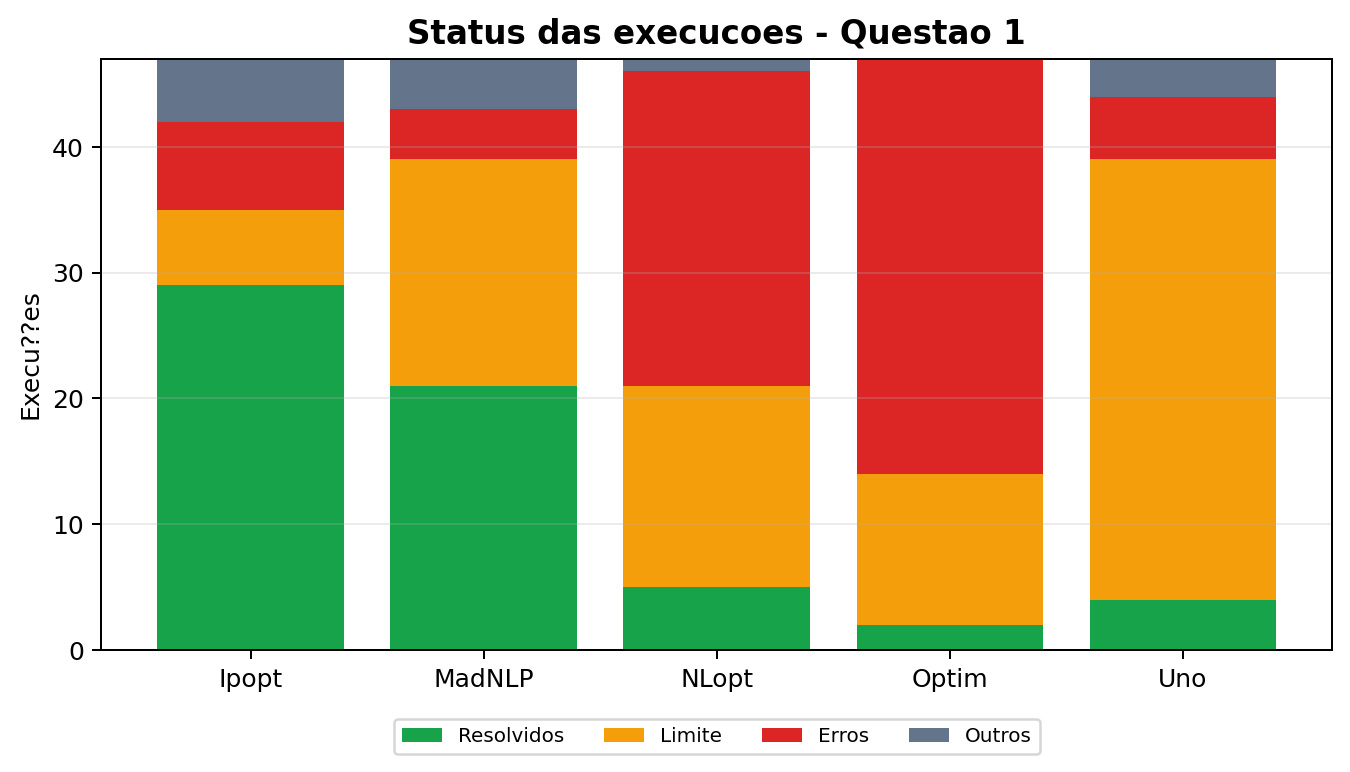
\includegraphics[width=0.86\textwidth]{figuras/integrado_status_q1.png}
\caption{Distribuicao dos status das execucoes da Questao 1.}
\label{fig:q1_status}
\end{figure}

\section{Resultados da Questao 2}

Na Questao 2, a etapa inicial consistiu em acessar a Library 1 da biblioteca COCONUT, identificar os problemas com valor objetivo de referencia definido, baixar os modelos GAMS e converter os arquivos selecionados para Julia/JuMP. A Tabela~\ref{tab:q2_preparacao} resume as etapas de preparacao.

\begin{table}[H]
\centering
\caption{Etapas de preparacao dos problemas da Questao 2}
\label{tab:q2_preparacao}
\begin{tabular}{lr}
\toprule
Etapa & Quantidade \\
\midrule
Problemas encontrados apos o filtro inicial & 202 \\
Arquivos GAMS baixados com sucesso & 188 \\
Falhas de download registradas & 14 \\
Problemas aprovados para conversao & 120 \\
Problemas convertidos para Julia/JuMP & 120 \\
\bottomrule
\end{tabular}
\end{table}

\begin{table}[H]
\centering
\caption{Falhas de download registradas na Questao 2}
\label{tab:q2_falhas_download}
\begin{tabular}{llll}
\toprule
ex7\_2\_5 & ex7\_2\_6 & ex7\_2\_7 & ex7\_2\_8 \\
ex7\_2\_9 & ex7\_2\_10 & ex8\_1\_8 & ex9\_1\_10 \\
ex9\_1\_3 & ex9\_1\_6 & ex9\_1\_7 & ex9\_1\_9 \\
ex9\_2\_1 & himmel11 & & \\
\bottomrule
\end{tabular}
\end{table}

A partir dos 120 problemas convertidos, cada modelo foi executado com Ipopt, MadNLP, NLopt, Optim e Uno. A Tabela~\ref{tab:q2_resumo} mostra o desempenho consolidado dos cinco solvers.

\begin{table}[H]
\centering
\caption{Resumo dos resultados da Questao 2: COCONUT GAMS}
\label{tab:q2_resumo}
\begin{tabular}{lrrrrrrr}
\toprule
Solver & Total & Resolvidos & Taxa (\%) & Limite & Erros & Outros & Tempo (s) \\
\midrule
Ipopt  & 120 & 105 & 87.5 & 1  & 1  & 13 & 412.39 \\
MadNLP & 120 & 103 & 85.8 & 1  & 1  & 15 & 638.15 \\
NLopt  & 120 & 101 & 84.2 & 17 & 2  & 0  & 5790.21 \\
Optim  & 120 & 86  & 71.7 & 2  & 32 & 0  & 1418.68 \\
Uno    & 120 & 68  & 56.7 & 3  & 15 & 34 & 1872.16 \\
\bottomrule
\end{tabular}
\end{table}

\begin{figure}[H]
\centering
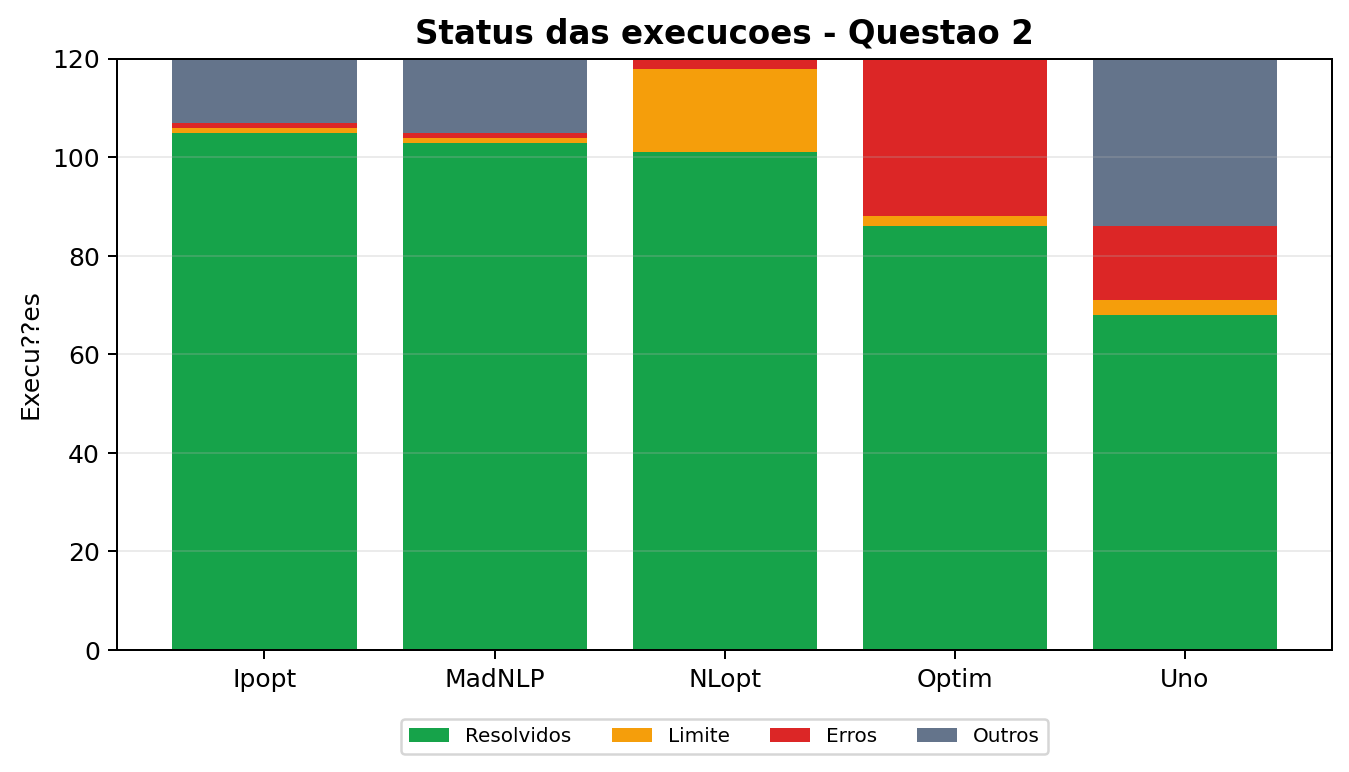
\includegraphics[width=0.86\textwidth]{figuras/integrado_status_q2.png}
\caption{Distribuicao dos status das execucoes da Questao 2.}
\label{fig:q2_status}
\end{figure}

\section{Comparacao Integrada}

Considerando as duas questoes, foram avaliados 167 problemas distintos, resultando em 835 execucoes solver-problema. A Tabela~\ref{tab:integrado} apresenta a comparacao integrada.

\begin{table}[H]
\centering
\caption{Resumo integrado das Questoes 1 e 2}
\label{tab:integrado}
\begin{tabular}{lrrrrrrrr}
\toprule
Solver & Total & Resolvidos & Taxa (\%) & Limite & Erros & Outros & Tempo (s) & Melhor obj. \\
\midrule
Ipopt  & 167 & 134 & 80.2 & 7  & 8  & 18 & 15724.99 & 88 \\
MadNLP & 167 & 124 & 74.3 & 19 & 5  & 19 & 40238.52 & 81 \\
NLopt  & 167 & 106 & 63.5 & 33 & 27 & 1  & 45980.99 & 64 \\
Optim  & 167 & 88  & 52.7 & 14 & 65 & 0  & 33820.00 & 54 \\
Uno    & 167 & 72  & 43.1 & 38 & 20 & 37 & 77281.23 & 61 \\
\bottomrule
\end{tabular}
\end{table}

O indicador ``melhor objetivo'' contabiliza, para cada problema, quais solvers obtiveram o melhor valor objetivo dentro da tolerancia adotada. Para problemas de minimizacao, o melhor valor corresponde ao menor objetivo encontrado entre os solvers validos; para problemas de maximizacao, corresponde ao maior valor. O gap absoluto foi calculado por
\[
Gap_{abs} = | f_{solver} - f_{ref} |,
\]
em que \(f_{solver}\) e o objetivo obtido pelo solver e \(f_{ref}\) e o melhor valor de referencia disponivel para comparacao.

\begin{figure}[H]
\centering
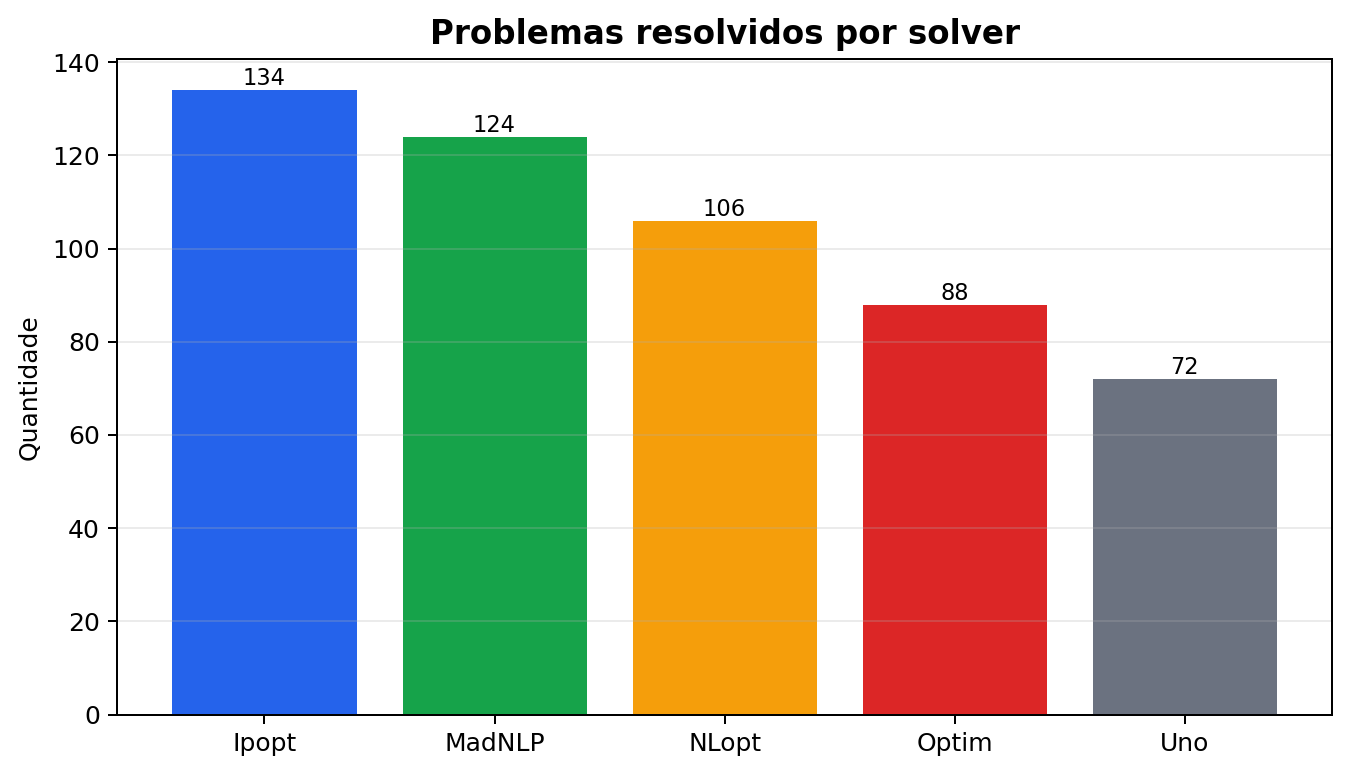
\includegraphics[width=0.82\textwidth]{figuras/integrado_grafico_resolvidos.png}
\caption{Quantidade integrada de problemas resolvidos por solver.}
\label{fig:integrado_resolvidos}
\end{figure}

\begin{figure}[H]
\centering
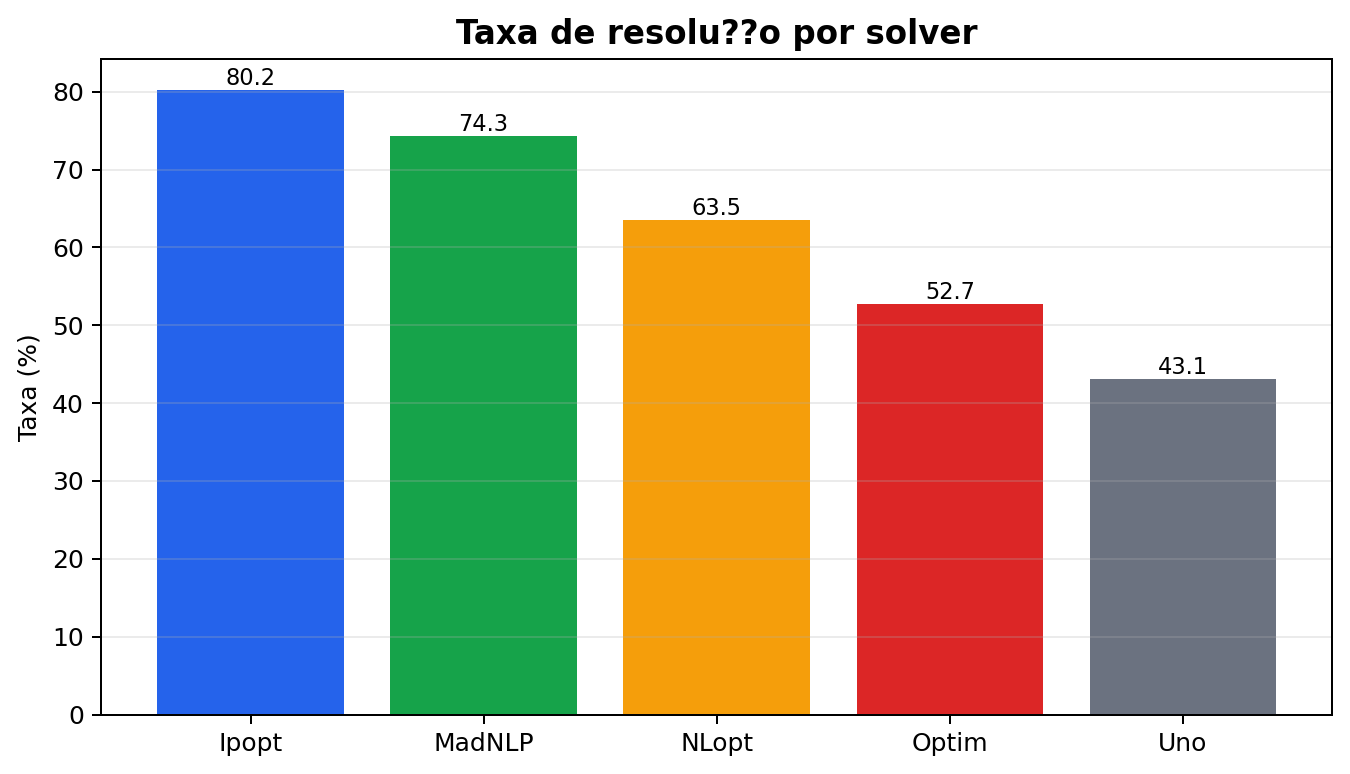
\includegraphics[width=0.82\textwidth]{figuras/integrado_grafico_taxa.png}
\caption{Taxa integrada de resolucao por solver.}
\label{fig:integrado_taxa}
\end{figure}

\begin{figure}[H]
\centering
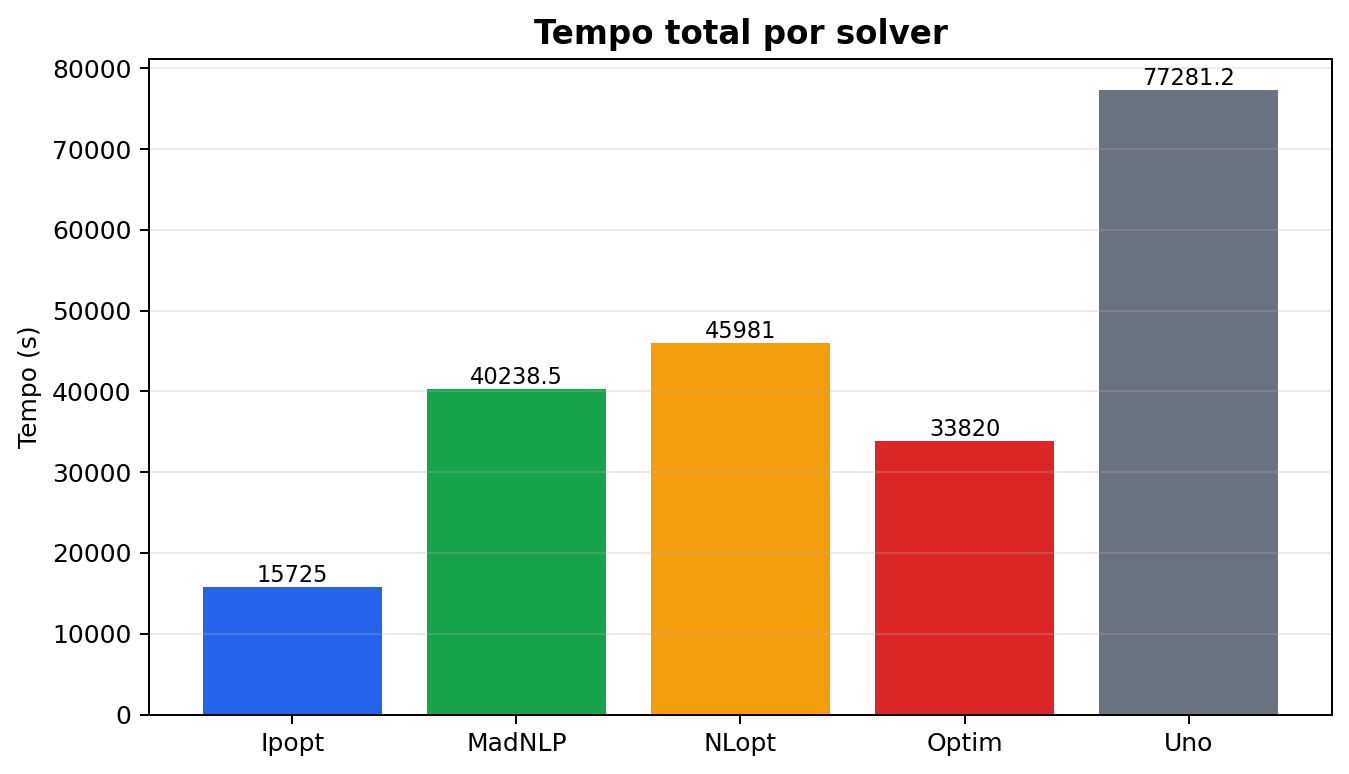
\includegraphics[width=0.82\textwidth]{figuras/integrado_grafico_tempo_total.png}
\caption{Tempo computacional total por solver.}
\label{fig:integrado_tempo}
\end{figure}

\begin{figure}[H]
\centering
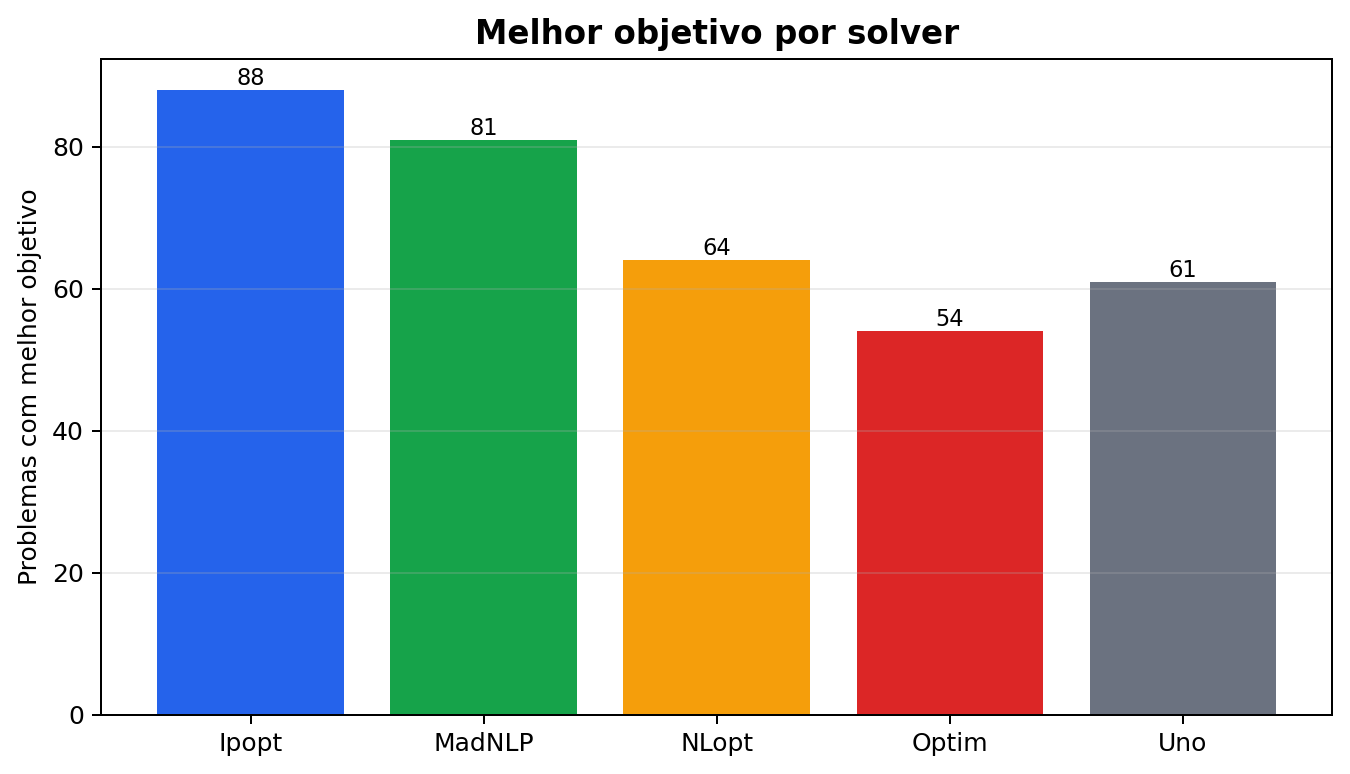
\includegraphics[width=0.82\textwidth]{figuras/integrado_grafico_qualidade.png}
\caption{Quantidade de melhores objetivos por solver.}
\label{fig:integrado_qualidade}
\end{figure}

\begin{figure}[H]
\centering
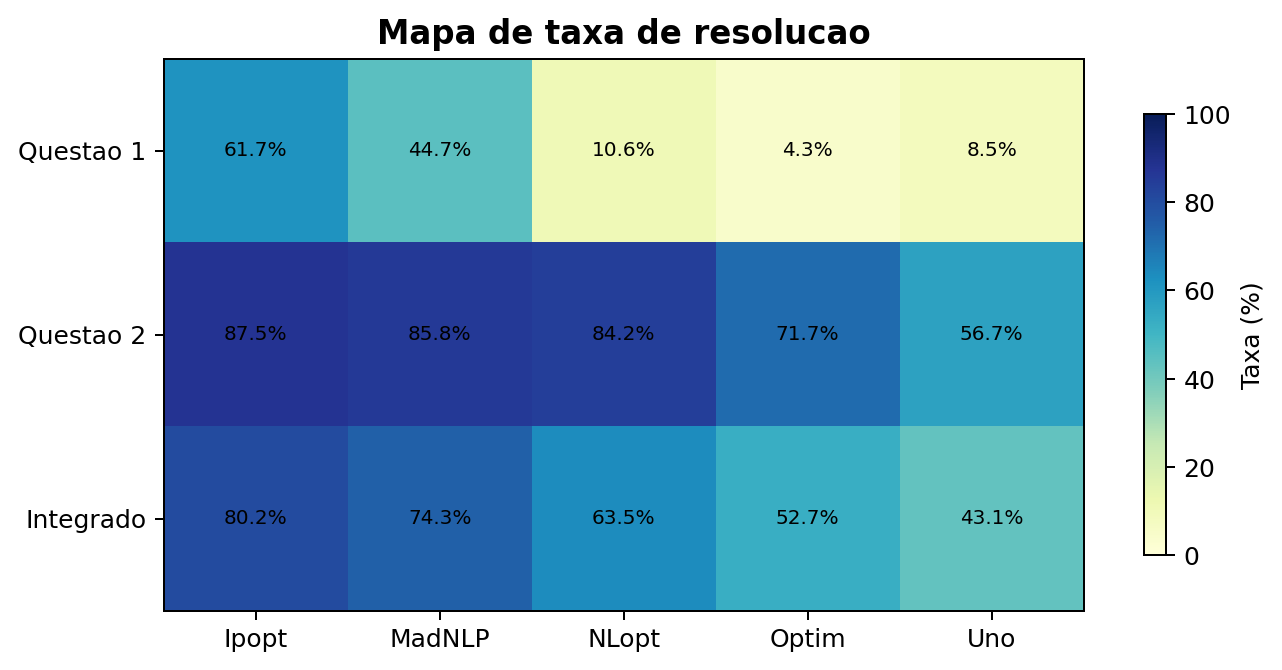
\includegraphics[width=0.88\textwidth]{figuras/integrado_heatmap_taxa.png}
\caption{Mapa comparativo das taxas de resolucao.}
\label{fig:integrado_heatmap}
\end{figure}

\section{Conclusao}

Nos resultados consolidados, Ipopt apresentou a maior taxa de resolucao integrada, com 134 problemas resolvidos entre 167, seguido por MadNLP, com 124 resolucoes. Na Questao 2, todos os solvers obtiveram desempenho superior ao observado na Questao 1, indicando que os modelos convertidos a partir dos arquivos GAMS apresentaram melhor compatibilidade operacional com o fluxo Julia/JuMP utilizado. Em termos de robustez geral, Ipopt e MadNLP foram os solvers mais consistentes. NLopt apresentou bom desempenho na Questao 2, mas menor robustez na Questao 1. Optim e Uno apresentaram maior quantidade de erros, limites de tempo ou classificacoes nao resolvidas.

\begin{thebibliography}{9}

\bibitem{plato}
H. D. Mittelmann, ``AMPL/NLP test problems,'' PLATO/ASU Optimization Test Problems. Disponivel em: \url{https://plato.asu.edu/ftp/ampl-nlp.html}.

\bibitem{coconut}
A. Neumaier, ``COCONUT Benchmark Library 1,'' Global Optimization Benchmark. Disponivel em: \url{https://arnold-neumaier.at/glopt/coconut/Benchmark/Library1_new_v1.html}.

\bibitem{jump}
JuMP Developers, ``JuMP.jl Documentation,'' Disponivel em: \url{https://jump.dev/JuMP.jl/stable/}.

\end{thebibliography}

\end{document}
